\documentclass[12pt]{article}

%Packages
\usepackage[a4paper, margin=1in]{geometry}
\usepackage{hyperref}
\usepackage{amsmath, amssymb}
\usepackage{booktabs}
\usepackage{indentfirst}
\usepackage{siunitx}
\usepackage{romannum}
\usepackage{multirow}
\usepackage{graphicx}
\usepackage{float}
\usepackage{titlesec}
\usepackage{tikz}
\usetikzlibrary{shapes.geometric, arrows, positioning}
\usepackage[american]{circuitikz}
\usepackage{bookmark}

\newcommand*{\titleGP}{\begingroup
	\centering % Center all text
	\vspace*{\baselineskip} % White space at the top of the page

	\rule{\textwidth}{1.6pt}\vspace*{-\baselineskip}\vspace*{2pt} % Thick horizontal line
	\rule{\textwidth}{0.4pt}\\[\baselineskip] % Thin horizontal line
	{\LARGE PH3144 | Electronics with Lab}\\[0.2\baselineskip] % Title
	\rule{\textwidth}{0.4pt}\vspace*{-\baselineskip}\vspace{3.2pt} % Thin horizontal line
	\rule{\textwidth}{1.6pt}\\[2\baselineskip] % Thick horizontal line

	\vspace*{1in}
    
    \LARGE Precision Closed-Loop AC Power Controller using PID 
    \vspace*{1in}\\
    
	\LARGE Group \#23\\
	\vspace*{1in}

	\Large Uday Pratap Bais (20231267)\\
	\vspace*{0.2in}
	\Large Yash Dadhwal (20231287)\\
	\vspace*{0.2in}
	\Large Yojit Kumar (20231289)\\
	\vspace*{0.2in}
\endgroup}

\makeatletter
\let\latexps@plain\ps@plain
\newcommand{\frontmatter}{\let\ps@plain\ps@empty\pagestyle{empty}}
\newcommand{\mainmatter}{%
  \let\ps@plain\latexps@plain\pagestyle{plain}%
  \clearpage
  \pagenumbering{arabic}}
\makeatother

\begin{document}
\frontmatter
\titleGP
\clearpage

\mainmatter
\section{Introduction}
\subsection{Background}
In modern electrical systems, precise control of power delivered to a load is essential for efficiency, stability, and protection of devices. One effective technique for regulating AC power is phase angle control, where the firing angle of a thyristor (SCR/triac) is adjusted to control the portion of the AC waveform delivered to the load. However, phase angle control by itself can lead to overshoot, slow response, or instability when load or input conditions vary.

To overcome these challenges, we propose the integration of a PID (Proportional– Integral– Derivative) controller. The PID algorithm dynamically adjusts the firing angle of the power electronics device based on feedback (such as load voltage, current, or power), ensuring that the output closely follows the desired setpoint. This combination allows us to achieve smooth, accurate, and stable power regulation in AC circuits.

\subsection{Objectives}
\begin{itemize}
\item Design and build a safe, isolated circuit for measuring real-time AC voltage and current.

\item Implement a phase angle control circuit using a Triac for regulating AC power.

\item Integrate these systems with an Arduino microcontroller.

\item Implement and tune a PID control algorithm to maintain a precise power setpoint.

\item Develop a user interface for setting the target power and viewing system status.
\end{itemize}

\section{Methodology}
%circuit diagrams and hardware implementation explanation
%logic diagrams and flowcharts

\subsection{Overview with Major Components}
\begin{figure}[h!]
\centering
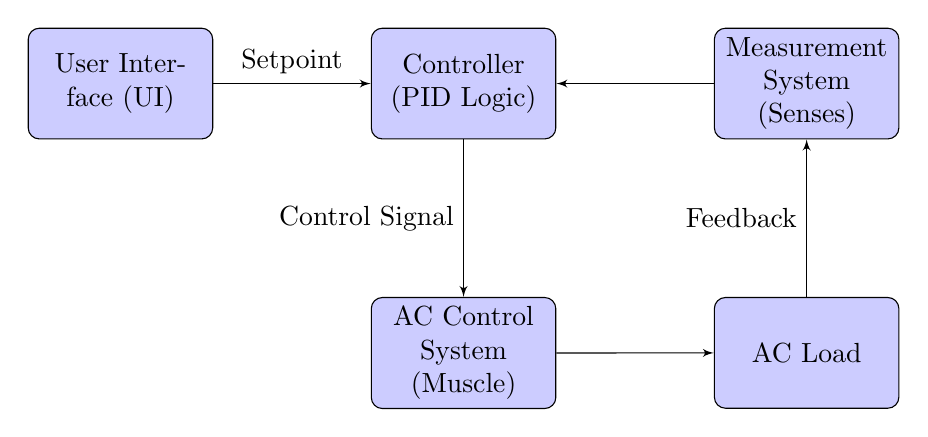
\begin{tikzpicture}[
    auto,
    block/.style={rectangle, draw, fill=blue!20, text width=6em, text centered, rounded corners, minimum height=4em},
    line/.style={draw, -latex'}
]

% Place the nodes
\node [block] (ui) {User Interface (UI)};
\node [block, right=2cm of ui] (arduino) {Controller (PID Logic)};
\node [block, below=2cm of arduino] (control) {AC Control System (Muscle)};
\node [block, right=2cm of arduino] (measure) {Measurement System (Senses)};
\node [block, below=2cm of measure] (load) {AC Load};

% Draw the lines (arrows)
\path [line] (ui) -- node [above] {Setpoint} (arduino);
\path [line] (arduino) -- node [left] {Control Signal} (control);
\path [line] (control) -- (load);
\path [line] (load) -- node [left] {Feedback} (measure);
\path [line] (measure) -- (arduino);

\end{tikzpicture}
\caption{System Overview of the Closed-Loop Power Controller}
\label{fig:block_diagram}
\end{figure}

\subsection{Circuit Diagrams}
\subsubsection{User Interface}
\begin{figure}[H]
\centering
\begin{circuitikz}[scale=1.1, every node/.style={scale=0.9}]
    
    % Title
    \node at (6,8) {\textbf{User Interface Module}};
    
    % I2C LCD Display
    \draw[thick] (2,6) rectangle (8,7.5);
    \node at (5,6.75) {\textbf{16x2 I2C LCD Display}};
    
    % LCD Connection pins
    \draw (2,7.2) to[short, *-] ++(-1,0) node[left]{SCL};
    \draw (2,6.8) to[short, *-] ++(-1,0) node[left]{SDA};
    \draw (2,6.4) to[short, *-] ++(-1,0) node[left]{VCC (+5V)};
    \draw (2,6.0) to[short, *-] ++(-1,0) node[left]{GND};
    
    % Push Button Section
    \node at (5,4.5) {\textbf{Set Point Control Buttons}};
    
    % UP Button Circuit
    \draw (1,3.5) node[vcc](vcc_up){+5V} to[short] ++(1,0) 
          to[push button, l=UP] ++(2.5,0) coordinate(up_out);
    \draw (up_out) to[short, *-] ++(1.5,0) node[right]{D5};
    \draw (up_out) to[R, l=$R_1$ 10k$\Omega$] ++(0,-1) node[ground](gnd_up){};
    
    % DOWN Button Circuit  
    \draw (1,1.5) node[vcc](vcc_down){+5V} to[short] ++(1,0) 
          to[push button, l=DOWN] ++(2.5,0) coordinate(down_out);
    \draw (down_out) to[short, *-] ++(1.5,0) node[right]{To Arduino D6};
    \draw (down_out) to[R, l=$R_2$ 10k$\Omega$] ++(0,-1) node[ground](gnd_down){};
    
    % Arduino Connection Summary Box
    \draw[dashed] (9,2.5) rectangle (13,6);
    \node at (11,5.5) {\textbf{Arduino Connections}};
    \node at (11,5) [align=left] {SCL → A5};
    \node at (11,4.6) [align=left] {SDA → A4};
    \node at (11,4.2) [align=left] {UP Button → D5};
    \node at (11,3.8) [align=left] {DOWN Button → D6};
    \node at (11,3.4) [align=left] {VCC → +5V};
    \node at (11,3) [align=left] {GND → GND};
    
\end{circuitikz}
\caption{User Interface Module - LCD Display and Control Buttons}
\label{fig:ui_circuit_improved}
\end{figure}

\subsubsection{AC Control System}

\begin{figure}[H]
\centering
\begin{circuitikz}[scale=1, every node/.style={scale=0.7}]
    
    % HIGH VOLTAGE SECTION - AC Input Lines
    \draw (0,5) node[left]{230V AC Live} to[short] ++(1,0) coordinate(live_in);
    \draw (0,4) node[left]{230V AC Neutral} to[short] ++(1,0) coordinate(neutral_in);
    
    % BTA416 Triac - draw as box with three connections
    \draw (live_in) to[short] ++(1,0) to[short,-*] ++(0,1) coordinate(triac_input);
    \draw (1.5,6) rectangle ++(2,1) coordinate(triac_box);
    \node at ([xshift=-1cm, yshift=-0.5cm]triac_box) {BTA416};
    
    % Triac connections
    \draw (triac_input) ++(1,0) to[short,*-] ++(0,-1) to[short] ++(1,0) coordinate(load_in);
    \draw (triac_input) ++(0.5,0) to[short,*-] ++ (0,-3) coordinate(gate);
    
    % Connect triac terminals
    \draw (load_in) to[lamp] ++(3,0) coordinate(after_load);
    \draw (neutral_in) to[short] ++(6,0) to[short] ++(0,1) coordinate(neutral_after load);
    
    % LOW VOLTAGE SECTION - Arduino connections
    \draw (0,1.5) node[left]{A9} to[short] ++(1,0) coordinate(arduino_pin);
    \draw (0,1) node[left]{VCC} to[short] ++(1,0) coordinate(arduino_5v);
    \draw (0,0.5) node[left]{GND (Arduino)} to[short] ++(1,0) coordinate(arduino_gnd);
    
    % MOC3023M Optoisolator input
    \draw (arduino_pin) to[R=\SI{330}{\ohm}] ++(1,0) to[short,-*] ++(0.5,0) coordinate(led_anode);
    \draw (arduino_5v) to[short,-*] ++(1.5,0) coordinate(5v_in);
    \draw (arduino_gnd) to[short,-*] ++(1.5,0) coordinate(gnd_in);
    
    % MOC3023M Optoisolator - draw as box with side connections
    \draw ([yshift=0.5cm]led_anode) rectangle ++(2,-2) coordinate(opto_box);
    \node at ([xshift=1cm, yshift=-0.5cm]led_anode) {MOC3023M};
    
    
    % Output side connections (right side of box)
    \draw (5v_in) ++(2,0) to[short,*-] ++(0.5,0) to[short] ++(0,2) to[short] (gate);
    
\end{circuitikz}
\end{figure}

\subsubsection{Measurement System}
\begin{figure}[H]
\centering
\begin{circuitikz}[scale=1, every node/.style={scale=0.7}]
    
    % AC Input Lines
    \draw (0,8) node[left]{230V AC Live} to[short] ++(1,0) coordinate(live_in);
    \draw (0,7) node[left]{230V AC Neutral} to[short] ++(1,0) coordinate(neutral_in);
    
    % Section 1: ZMPT101B Voltage Module
    \draw[thick] (1,6.5) rectangle (4,8.5);
    \node at (2.5,7.8) {\textbf{ZMPT101B}};
    \node at (2.5,7) {\textbf{Voltage Module}};
    
    % ZMPT101B connections
    \draw (live_in) to[short] (0,8);
    \draw (neutral_in) to[short] (0,7);
    \draw (4,7.5) to[short] ++(1,0) coordinate(zmpt_out);
    \node at (4,7.7) [right] {Analog Out};
    \draw (5,7.5) to[short, *-] ++(0,-1) to[short,-*] ++(1,0) node[right] {A0};   
    
    % Section 2: SCT-013-030 Current Sensor
    \node at (4,4.5) {\textbf{SCT-013-030 Current Sensor}};
    
    % HIGH VOLTAGE SECTION - AC Input Lines (separated physically)
    \draw (0,3) node[left]{230V AC Live} to[short] ++(1,0) coordinate(live_in1);
    \draw (0,1.5) node[left]{230V AC Neutral} to[short] ++(1,0) coordinate(neutral_in1);
    
    % Live wire going to load (this is what the CT clamps around)
    \draw[ultra thick, red] (live_in1) to[short] ++(1,0) coordinate(live_to_load) 
          to[short] ++(2,0) coordinate(live_mid) to[lamp, l=Load] ++(3,0) 
          coordinate(live_after_load);
    \draw[thick, blue] (neutral_in1) to[short] ++(6,0) 
          to[short] ++(0,1.5) to[short] (live_after_load);
    
    % SCT-013-030 Current Transformer (clamps around live wire)
    \draw[thick] ([yshift=0.5cm]live_mid) arc (180:0:0.3) coordinate(ct_top_right);
    \draw[thick] ([yshift=-0.5cm]live_mid) arc (-180:0:0.3) coordinate(ct_bottom_right);
    \draw[thick] (ct_top_right) -- (ct_bottom_right);
    \node at ([yshift=-1cm]live_mid) {SCT-013-030};
    
    % LOW VOLTAGE SECTION - CT output leads (physically separated)
    \draw (ct_top_right) to[short] ++(0.5,0) coordinate(isolation_point1);
    \draw (ct_bottom_right) to[short] ++(0.5,0) coordinate(isolation_point2);
    
    % Jump across isolation barrier
    \draw (isolation_point1) to[short] ++(1,0) coordinate(ct_signal);
    \draw (isolation_point2) to[short] ++(0,-1) node[ground]{};
    
    % Voltage divider to create 2.5V DC offset
    \draw (ct_signal) to[short] ++(1.5,0) coordinate(signal_point);
    \draw (signal_point) to[short] ++(0,0.5) to[R, l=$R_1$ 10k$\Omega$] ++(0,1) 
          node[vcc](vcc1){+5V};
    \draw (signal_point) to[short] ++(0,-0.5) to[R, l=$R_2$ 10k$\Omega$] ++(0,-1) 
          node[ground](gnd1){};
    
    % Coupling capacitor and output
    \draw (signal_point) to[C, l=$C_1$ \SI{10}{\micro\farad},*-] ++(2,0) coordinate(arduino_current);
    \draw (arduino_current) to[short, -*] ++(1.5,0) node[right]{A1};
    
    % Section 3: Zero-Crossing Detector
    \node at (10.8,6) {\textbf{Zero-Crossing Detector}};
    
    % Input from ZMPT101B
    \draw (zmpt_out) to[short] ++(1,0) to[R, l=$R_{in}$ \SI{10}{\kilo\ohm}] ++(2,0) coordinate(zcd_input);
    
    % H11AA1 Optocoupler
    \draw[thick] (9.5,6.8) rectangle (11.5,8.2);
    \node at (10.5,7.5) {\textbf{H11AA1}};
    \draw (zcd_input) to[short] (9.5,7.5);
    \draw (9.5,7.1) to[short] ++(-0.5,0) to[short] ++(0,-1.5) node[ground]{};
    
    % Voltage divider for reference
    \draw (9,9) to[R, l=$R_3$ \SI{10}{\kilo\ohm}, *-] ++(2,0) node[vcc]{+5V};
    \draw (9,9) to[R, l=$R_4$ \SI{10}{\kilo\ohm}] ++(-2,0) node[ground]{};
    \draw (9,9) |- (9.5,7.9);
    
    % Output circuit
    \draw (11.5,7.9) to[short] ++(0.5,0) to[R, l=\SI{10}{\kilo\ohm}] ++(0,1.5) node[vcc, label=left:+5V]{};
    \draw (11.5,7.1) to[short] ++(1,0) to[short] ++(0,-1.5) node[ground]{};
    \draw (11.5,7.5) to[short, -*] ++(1,0) node[right]{A2};
    
    % Arduino connections summary
    \draw[dashed] (9.2,1.2) rectangle (13,3);
    \node at (11,2.8) {\textbf{Arduino Connections}};
    \node at (11.3,2) [align=left] {A0: Voltage Signal \\ A1: Current Signal \\ A2: Zero-Cross Interrupt};
    
    
\end{circuitikz}
\caption{Measurement and Timing Module Schematic}
\label{fig:complete_measurement_module_improved}
\end{figure}

\section{Challenges \& Troubleshooting strategy}
\subsection{Safety}
The project involves working with AC mains supply, which introduces several safety concerns. The foremost challenge is high voltage exposure, since direct contact with live components can cause severe electric shock or injury. To mitigate this, all high-voltage sections are enclosed, and isolation is provided between the control and power circuits.

Short circuits and overcurrent conditions are also possible due to load faults or wiring errors, leading to damaging current surges. To counter this, fuses and circuit breakers are employed to protect the circuit from catastrophic failure. Similarly, improper isolation between the high-voltage power stage and the low-voltage control circuitry poses the risk of leakage currents reaching the user or microcontroller. This issue is minimized by using opto-isolators, isolation transformers, and careful PCB layout design.

Another important aspect is the misuse or rating exceedance of components, where devices such as SCRs, triacs, or resistors may fail if operated beyond their current, voltage, or thermal limits. To avoid this, all components are chosen with appropriate safety margins.
\subsection{PID tuning}
Tuning a PID controller for AC power regulation using phase angle control presents several challenges. One of the main difficulties is the nonlinear relationship between firing angle and load power, since PID control generally assumes a linear system model. This mismatch makes it harder to achieve stable tuning. Another issue arises from system delays, particularly with inductive loads, which introduce phase lag and can cause oscillations or instability in the response. In addition, there is significant coupling between the parameters $K_p$, $K_i$, and $K_d$, such that adjusting one parameter often changes the effect of the others, making the tuning process less straightforward. The system is also vulnerable to noise in feedback signals, as voltage and current sensors can pick up switching noise from SCR or triac operations, which is especially problematic for the derivative term that tends to amplify high-frequency noise. Another challenge is integral windup, where prolonged errors cause the integral term to accumulate excessively, leading to overshoot and sluggish recovery. Finally, the controller’s performance can vary significantly under different load types, since gains tuned for resistive loads may not be suitable for inductive loads that respond more slowly.

\section{Summary}
This project undertakes the design and implementation of a Precision Closed-Loop AC Power Controller. Standard open-loop AC control methods, such as simple dimmers, are susceptible to inaccuracies caused by fluctuations in mains voltage and changing load conditions. To overcome this, our system will employ a closed-loop feedback mechanism driven by a Proportional-Integral-Derivative (PID) control algorithm.

The primary objective is to create a robust and stable system capable of maintaining a user-defined power setpoint with high precision, demonstrating a practical application of control theory in modern power electronics. Safety is a paramount design consideration, addressed through galvanic isolation between low-voltage logic and high-voltage power circuits.
\end{document}

